\documentclass{article}

%\renewcommand{\baselinestretch}{1.5}
\addtolength{\oddsidemargin}{-0.5in}
%\addtolength{\topmargin}{-0.2in}
\addtolength{\textheight}{0.2in}
\addtolength{\textwidth}{1in}

%%%
\usepackage[authoryear,round]{natbib}
%or (if you have an unshiny latex installation)
%\newcommand{\citep}[1]{{\{\sf#1\}}}
%%%
\usepackage{alltt}

%% Postscript fonts
\usepackage{times}
\usepackage{graphicx}

\ifx\pdfoutput\undefined
  %% Stuff wout hyperref
  \def\url#1{\textsf{#1}} % To help fit in lines
\else
  %% Stuff with hyperref
  \usepackage{hyperref}
  \hypersetup{backref,colorlinks=true,pagebackref=true,hyperindex=true}
\fi

%%---End of package requiring ---------- Own Definitions -------------

\newcommand*{\Splus}{\textsc{S-Plus}}
\newcommand*{\XLispStat}{\textsc{XLispStat}}
\newcommand*{\Stata}{\textsc{Stata}}
\newcommand*{\Rgui}{\textsc{Rgui}}
\newcommand*{\Fortran}{\textsc{Fortran}}
\newcommand*{\Scmt}[1]{\hbox{\qquad {\footnotesize \#\#} \textsl{#1}}}
\newtheorem{defn}{Definition}[section]
\newtheorem{ex}{Example}[section]

\newcommand{\stexttt}[1]{{\small\texttt{#1}}}
\newcommand{\ssf}[1]{{\small\sf{#1}}}
\newcommand{\elcode}[1]{\\{\stexttt{\hspace*{2em} #1}}\\}
\newenvironment{Salltt}{\small\begin{alltt}}{\end{alltt}}
\newcommand{\US}{{\char'137}}        % \tt _
\newcommand{\marpar}[1]{\marginpar{\raggedright#1}}
\newcommand{\file}[1]{`\stexttt{#1}'}

%%--------------------------------------------------------------- Start Text

\title{Emacs Speaks Statistics: A Universal Interface for
  Statistical Analysis}

\author{A.J. Rossini \and Martin M{\"a}chler \and Kurt Hornik \and Richard
  M. Heiberger \and Rodney Sparapani \footnote{%
%%
    A.J. Rossini is Research Assistant Professor in the Department of
    Biostatistics, University of Washington and Joint Assistant Member at
    the Fred Hutchinson Cancer Research Center, Seattle, WA, USA
    (E-mail: rossini@u.washington.edu);
%%
    Martin M{\"a}chler is Senior Scientist and Lecturer in the Seminar for
    Statistics, ETH Zurich, Zurich, Switzerland
    (E-mail: maechler@stat.math.ethz.ch);
%%
    Kurt Hornik is Professor in the Institut f{\"u}r Statistik,
    Wirtschaftsuniversit{\"a}t Wien and the Institut f{\"u}r
    Wahrscheinlichkeitstheorie und Statistik, Technische Universit{\"a}t
    Wien, Vienna, Austria (E-mail: Kurt.Hornik@r-project.org);
%%
    Richard M. Heiberger is Professor in the Department of Statistics at
    Temple University, Philadelphia, PA, USA (E-mail: rmh@temple.edu);
%%
    and Rodney Sparapani is Senior Biostatistician at the Medical College
    of Wisconsin, Milwaukee, WI, USA (E-mail: rsparapa@mcw.edu)}}

\date{\today}

\begin{document}

\maketitle

Keywords: Data Analysis, Programming Tools, User Interfaces, SAS,
\Splus, R, \XLispStat, \Stata

\begin{abstract}
  Emacs Speaks Statistics (ESS) is a user interface for developing
  statistical applications and performing data analysis using any of
  several common statistical programming languages.  ESS falls in the
  programming tools category of Integrated Development Environments
  (IDEs), which are approaches for developing and visualizing computer
  programs.  We discuss how it works, the advantages of using it, and
  extensions for increasing statistical programming efficiency.
\end{abstract}

\baselineskip=2pc

\section{Introduction}
\label{sec:intro}

Integrated Development Environments (IDEs) are computer programming
environments which combine features and tools in a single interface
with the intent of increasing programmer productivity and efficiency.
In the last decade, the use of IDEs and other Rapid Application
Development (RAD) tools has shortened the development time of complex
software systems with programming languages such as Visual Basic,
Java, C++, Python, and Smalltalk.  For the field of statistics,
programming is an important skill which can be augmented and enhanced
by the right tools and environment.  This is especially important with
the increased use of simulation-based statistical procedures including
resampling and Markov Chain Monte Carlo (MCMC) sampling.

Statistical software tools are intended for either general data
analysis or for specialized forms of statistical analyses.  The
specialized tools can be orders of magnitude more efficient for
generating data analyses.  This is balanced by the inability of the
specialized tools to perform a wide range of common data analysis
operations.  Tightly coupled interoperability between these programs
rarely exists, while the need to switch between tools occurs much more
often.  For example, general purpose tools such as R
\citep{ihak:gent:1996} do not perform Bayesian analyses as easily as
tools such as WinBUGS can \citep{SpieThomBest:1999}.  On the other
hand, these specialized tools lack breadth in the range of analyses
and graphics that can be generated.  For this reason, BUGS is
distributed with applications providing loose interoperability for
simplifying the transfer of output to R or \Splus{} for processing the
results.  Although the interfaces for WinBUGS and R are similar,
they are distinct enough to create tension on the part of the
analyst.

Emacs Speaks Statistics (ESS) \citep{ESS} is an extension package for
the Emacs editor which provides a single interface for a variety of
statistical computing tasks.  ESS is optimized for statistical coding
and interactive data analysis.  Statistical coding is the writing of
computer code for data analysis.  This code might be in a compiled
language, such as C or \Fortran, or it might be in an interpreted
language such as \Splus, SAS, R, \XLispStat, Perl, or Python.
Entering commands for interactive data analysis is a similar activity.
In either case, text is written in a computer language and sent to a
computer program for evaluation.  The primary difference is that the
results of a small set of commands are of critical interest for review
in the analysis phase, but the results of all commands are of interest
in the coding phase.  Both of these tasks can occur simultaneously,
for example in the use of compiled C code for optimization, which is
called from an interpreted language such as R, where the objective
function to optimize is written.

Simple conflicts between interfaces are exemplified by different
keystrokes for editing tasks such as copy and paste, beginning of
line, highlighting regions.  These are sometimes the most aggravating
because our fingers are trained for a primary interface convention
which is continually interfered with.  ESS solves this problem by
providing a uniform keyboard interface.

Complex conflicts between interfaces can involve the coordination of
several data files, multiple statistical software packages, and the
corresponding source code in each of these languages, combined for a
single analysis.  ESS, as part of Emacs, has tools which assist in
this, including support for version and source code control systems,
tools for accessing programs or files on remote machines, and
interfaces to documentation systems including \LaTeX\ and
\textsc{xml}.  In addition, Emacs can assist with, or be programmed to
perform, many tasks related to data cleaning, management, and editing.

It can be useful to have multiple statistical processes running
simultaneously, either on a single machine or a variety of machines.
This capability assists with code design and testing across multiple
versions of statistical software packages, as well as large scale
numerical simulations.  For example, one might want to be connected to
multiple R processes of different versions in order to verify behavior
on different versions of the same software; multiple processes of the
same version to perform test-and-run scenarios where one process is
doing long-term processing while the other is doing short-term
testing; simulations; and to distribute the load over a variety of
remote machines.

ESS mitigates some of the problems noted above.  It provides a well
designed and documented programming editor, an interface to
statistical processes, and provides, through Emacs, additional tools
which aid both statistical software development and data analysis.  It
works with common statistical software, including the S languages
(which include S \citep{BecRCW88,ChaJH92,ChaJ98}, \Splus{}
\citep{Splus}, and R \citep{ihak:gent:1996}); \XLispStat\
\citep{Tier90} and its extensions Arc \citep{Cook:Weisberg:1999} and
ViSta \citep{youn:fald:mcfa:1992}; SAS \citep{SAS:8.0}; \Stata\
\citep{Stata:6.0}; Omegahat \citep{DTLang:2000}; and BUGS
\citep{SpieThomBest:1999}.  ESS can be extended to accommodate most
statistical packages which can be controlled from a command-line.

The present paper is intended as the primary historical and
non-technical description of ESS.  A general paper with some user
how-to/FAQ information appears in \citep{heiberger:dsc:2001}.  Details
on the functions within ESS and examples of its use are included in
the online documentation that comes with the package.  The next
section introduces common forms of statistical user interfaces.  This
is followed by a discussion of ESS and Emacs.  Specifics on the
realized interfaces for the S family and SAS are discussed in sections
\ref{sec:S} and \ref{sec:SAS} respectively.  The conclusion
brings up related work and future extensions.

\section{Statistical User Interfaces}
\label{sec:UI}

Human interfaces for statistical packages and languages can generally be
classified into 3 forms, the command-line interface, the graphical user
interface, and a catch-all category for specialized interfaces which
only have 1 or 2 examples.  Command-line interfaces (CLIs) have
historically been used by many packages.  This is the interface that ESS
uses for control and provides a limited interface for.  Modern
statistical packages have generally used graphical user interfaces
(GUIs), sometimes exclusively.  In addition, there have been many
single-implementation interfaces, including flow-chart guides,
implemented as graph-based interfaces in ViSta \citep{youn:lubi:1995};
the SAS terminal interface, which divides the terminal window into 3
screens; and the coherent implementation provided by DataDesk
\citep{vell:prat:1989}, which has a tight link between data and
graphics.

Computer users strongly resist changes to their interface.  This can be
observed in the choice of editors such as vi and emacs; mail user agents
such as mail, Pine, Elm, Netscape Mail, and Microsoft Outlook; word
processors such as Microsoft Word and Corel WordPerfect; and other
commonly used tools.  The user's choice has little to do with theory,
and more to do with compatibility with previous usage and with
perceived size of the learning curve for a new package.
However, sometimes the hardest
interfaces to master are the most efficient in the long run---after the
initial investment in time.

\subsection{Command line interfaces}
\label{sec:UI:command}

The CLI is available for many statistical packages, particularly those
that were originally developed under Unix, MS-DOS, and
mainframe computers.  The CLI is the successor to the IBM punch-card
based batch interface.  The CLI consists of entering
commands one line at a time.  Current examples
are \Splus, R, \Stata, and \XLispStat.  Note that
the \Stata\ CLI is deprecated in favor of a new GUI, and this
direction seems to be a general trend.  We note that SAS does not have
a true CLI.  The two possible options for SAS are a prompt-less input
device which sends a combined log and list-file text stream directly
back to the same device, and second, the classic 3-window %graphical
terminal interface which is being deprecated in favor of a GUI
version.

\subsection{Graphical User Interfaces}
\label{sec:UI:GUI}

The advent of Apple Macintosh (Mac) and Microsoft Windows (Windows)
operating systems have encouraged a partial standardization of
interfaces for statistical packages.  Many packages written for both Mac
and Windows personal computers have adopted a data display descended
from the spreadsheet data-table approach.  Generally, these feature a
cases-by-variables spreadsheet representation of the data, along with
pull-down menus and dialog boxes for data analysis activities.
Depending upon their nature, numerical results can be saved as well as
displayed on the spreadsheet.  Statistical software packages that take
this basic approach include SPSS, Minitab, \Splus{} (4.x for Windows and
6.x for Unix and Windows), DataDesk, and ViSta.

Most statistical software, including spreadsheets, use the Multiple
Document Interface (MDI).  This user interface style encloses multiple
views of text, figures, and toolbars enclosed by the surrounding
application.  The use of MDI seems to be more a function of the
availability of GUI toolkits for Mac and Windows applications, which
promote such interfaces, rather than a consistent choice based on
theories for user-interface design.  The common approach taken by
statistics packages for MDI is to wrap menus and toolbars around a
region containing representations of documents.  These representations
usually include one or more frames possibly featuring display
graphics, a command-line window, a source code editing window, or
possibly a spreadsheet displaying, for example, a cases-by-variables
view of the data set or a drill-down contingency table interface.
This approach is employed by both spreadsheet packages such as
Microsoft Excel as well as most Mac and Windows statistical packages
including \Splus{} and SPSS.

The Single Document Interface (SDI) provides a single frame for each
document, view, or figure created.  Unix-based interfaces tend to be
SDI-based, due in part to the nature of the X11 windowing system---with its
flexibility in allowing a single application to place frames and
windows across multiple displays on potentially multiple computers---and
in part to the lack until recently of available GUI toolkits which
worked across different Unix platforms.  Examples of statistics
packages using the SDI are the command-line interfaces for \Stata,
\Splus, \XLispStat, or R under Unix and the \Rgui\ interface for R
under Windows.  In each of these the terminal window is considered to
be one document and the graphics displays to be the other parts of an
overall GUI.


\section{The ESS user interface}
\label{sec:ESS}

ESS extends Emacs by providing a number of features for statistical
programming.  This is done by extending the editor to provide
additional useful features, and in the case of interactive statistical
programs, sitting ``in front of'' their CLI and intercepting and
modifying I/O as needed.  We describe the exact features more in this
section.  

%% change/edit
Figure~\ref{fig:1} provides an example of how it looks when being used
with XEmacs.  This screenshot shows both SAS and R code being examined
at the same time, with an R interactive process being controlled from
within XEmacs.

Figure~\ref{fig:2} shows ESS running in NTemacs 21.0 on Windows 2000.
We are currently displaying 6 buffers.  \stexttt{highlight.s}
illustrates several uses of syntactic highlighting.
The most glaring one is the bright purple indicator for the
unbalanced parentheses.
We also see color choices for  keywords (\stexttt{if}), comments,
and quoted strings.  The string on the last line was not properly
terminated and we are immediately warned by the string color staying
on through (what we think is) the end of the line.

The two buffers \stexttt{transcript-before.st} and
\stexttt{transcript-after.st} show transcript editing.  A single ESS
command converted the before buffer into the after buffer by removing
all lines that do not begin with a prompt character.

The last three buffers show that a single S language source file can
be used with two (or more) executing processes.  In this example we
sent over first a subset of the line in \stexttt{tmps.s} and then the
entire line to the instance of S+4 running in an inferior
\stexttt{iESS(Sqpe)} buffer.  The we switched the connection to send
the same line to the instance of R running in the \stexttt{iESS(R)}
buffer.  The dialog about the process switch appears in the message line.


\subsection{Features and capabilities}
\label{sec:ESS:features}

Since ESS originated as S-mode, which provided an interface for
programming and process control under GNU Emacs for \Splus\ version 3,
ESS strongly supports the S family of languages; these include recent
versions of S, \Splus, and R.  SAS is also well supported.  \Stata\
and \XLispStat\ (and the \XLispStat\ extensions, ARC and ViSta) are
supported with the basic functionality of syntax highlighting and
process-interfacing.  ESS and its interface are fully discussed in the
next section.

\paragraph{Syntactic indentation and color/font-based source code
  highlighting.}
The ESS interface includes a description of the syntax and grammar of
each statistical language it knows about.  This gives ESS the ability
to edit the programming language code, often more smoothly than with
editors distributed with the languages.  The process of programming
code is enhanced as ESS provides the user with a clear presentation of
the code with syntax highlighting to denote assignment, reserved
words, presence of strings, and comments.  ESS has customizable
automatic indentation, with the customization based on the syntactic
structure of groups of expressions.  ESS knows the structure of
transcripts of the executing session and provides syntactic highlighting
for transcripts.  ESS interacts well with the executing statistics
language/program and
provides means for searching the command-line history for previous
commands and editing them for current use.

\paragraph{Partial code evaluation.}
Emacs can send individual lines, entire function definitions, marked
regions, and whole edited buffers from the window in which the code is
displayed for editing to the statistical language/program for
execution.  Emacs can complete partially typed file names by referring
to the current working directory.  Emacs sends the code directly to
the running program and receives the printed output back from the
program.  This is a major improvement over cut-and-paste as it does
not require switching buffers or windows.  The response is
received immediately in an editable Emacs buffer.

\paragraph{Object name completion.}
In addition, for languages in the S family (S
developed at Bell Labs, \Splus, and R)
ESS provides object-name completion of both user- and system-defined
functions and data.  ESS can dump and save
objects (user- and system-generated) into text files in a formatted
manner for editing, and reload them (possibly after editing) back
into the statistical language/program.

\paragraph{Source code checking.}
ESS facilitates the editing of source code by providing a means for
loading and error-checking of small sections of code for S,
\XLispStat, and SAS.  This allows for source-level debugging of batch
files.

\paragraph{Process interaction.}
Emacs has historically referred to processes under its control as
``inferior'', accounting for the name inferior ESS (\stexttt{iESS}) to
denote the mode for interfacing with the statistical package.  The
output of the package goes directly to an editable text buffer in Emacs.
This mode allows for command-line editing and saving history, as well as
recalling and searching for previously entered commands.  Filename
completion is available.  In addition (currently only for S languages),
there exists object-name and function-name completion.  Transcripts are
easily recorded and can be edited into an ideal activity log which can
then be saved.  There is a good interface for handling and intercepting
calls to the internal help systems for S, \XLispStat, and \Stata.

\paragraph{Interacting with statistical programs on remote computers.}
ESS provides the facility to edit and run programs on remote machines
in the same session and with the same simplicity as if they were
running on the local machine.  The remote machine could be a very
different platform than the local machine.

\paragraph{Transcription Editing and Reuse.}
Once a transcript log is generated, perhaps by saving an \file{iESS}
buffer, transcript-mode assists with reuse of part or all of the
entered commands.  It permits editing and re-evaluating the commands
directly from the saved transcript.  This is is useful for
demonstration of techniques as well as for reconstruction of data
analyses.  There currently exist functions within ESS for cleaning
transcripts from S languages back to source code by finding all input
lines and isolating them into an input file.

\paragraph{Help File Editing (R).}
ESS also provides an interface for writing help files for R functions
and packages.  It provides the ability to view and execute embedded R
source code directly from the help file in the same manner as ESS
normally handles code from a source file.  \stexttt{Rd} mode provides
syntax highlighting and the ability to submit code to a running ESS
process, either R or \Splus.

\subsection{Emacs}
\label{sec:ESS:emacs}

Emacs \citep{RMS:2000} is a mature, powerful, and easily extensible
text editing system which while traditionally used under Unix, is
freely available under the GNU General Public License for a large
number of platforms, including Unix, Mac, and Windows.  Emacs shares
some features with word processors, and more importantly, shares many
characteristics with operating systems.  Most importantly, Emacs can
interact with and control other programs either as subprocesses or as
cooperating processes.

Recent versions of Emacs commands provide both a GUI and terminal
interface which can respond to both keyboard and mouse usage.  The
mouse-based interface, through menus and toolbars (toolbars available
currently with XEmacs), tries to facilitate the learning of
keystroke-based short-cuts.  User-defined additional menus and
toolbars can be constructed as needed.

Emacs provides facilities that go beyond simple insertion and
deletion: viewing two or more files at once; editing formatted text;
visual comparison of two similar files; and navigation in units of
characters, words, lines, sentences, paragraphs, and pages.  Emacs
knows the syntax of each programming language.  It can provide
automatic indentation of programs and highlight with fonts or colors
specified syntactic characteristics.  Emacs is extensible using a
dialect of Lisp \citep{RChassell1999,PGraham:1996}.  This means that
new functions, with user interaction, can be written for common and
repeated text-editing tasks.

Most programming and documentation tasks fall under the realm of text
editing.  This work can be enhanced by common IDE features such as
contextual highlighting and recognition of special reserved words
appropriate to the programming language in use.  In addition, editor
behaviors such as folding, outlining, and bookmarks can assist with
maneuvering around a file.  Type-setting and word-processing, which
focus on the presentation of a document, are tasks that are not pure
text-editing.  Emacs shares many features with word-processing
programs and cooperates with document preparation systems such as
(\LaTeX; SGML, \textsc{xml}, and XSLT; and Noweb).

The capabilities can be extended in an orthogonal manner to include
other Emacs packages for assisting with documentation as noted above;
version control (RCS, CVS, SCCS, PRCS); and remote editing via FTP or
secure transport mechanisms such as ssh and scp.  Emacs handles the
interface to both source code and transcripts contextually, providing
syntax highlighting, bookmarking features, interfaces to directory
structure, and command-history.  Other extensions to Emacs allow it to
act as a World-Wide-Web browser, a highly sophisticated mail and news
reader, a shell/terminal window with history, and as an interface to
other common text-based tools such as spell checking programs.  The
Emacs keyboard and mouse interface can be re-mapped to resemble that
of other text-editors, such as ed, vi, wordstar, and brief.

The above reasons suggest that Emacs is a reasonable starting choice
for providing a universal interface for data analysis and programming.
ESS extends Emacs to provide a functional, easily extensible and
uniform interface for multiple statistical packages.

\subsection{History of ESS}
\label{sec:ESS:history}

ESS is an example of how open-source products can continue to develop
beyond what their initial authors planned.  The ESS codebase was brought
to life in 1989 initially as S-mode, to provide extensions to Emacs for
editing S and \Splus{} files.  This was originally written by Doug
Bates, Ed Kademan, Frank Ritter, and Mike Meyer.  David Smith was the
next primary maintainer, and his most important contribution was to
enhance the interface to the \Splus{} command-line interface and to
allow for control of multiple processes simultaneously.  In 1995, A.J.
Rossini extended S-mode to support XEmacs, an open-source editor which
was derived from Emacs.  At the same time, extensions from ETH, written
by Martin M{\"a}chler, were folded into what was to become the primary
codebase.  By 1996 a uniform S-mode, available for both Emacs and
XEmacs, supported S, \Splus, and to some extent R.  Kurt Hornik was
instrumental in enhancing support for R, in particular providing Rd
mode.

The other ancestor of the ESS codebase was a successful SAS-mode
written by Tom Cook.  The initial extension was done by A.J. Rossini
in 1995 to work with XEmacs, and this provided the initial impetus to
provide a uniform codebase for statistical programming.

The extension to a language-independent generic interface was prompted
by the success of R, and the need for an R-mode.  This led to a merger
with the SAS-mode \citep{SASMODE}, and the refactoring of the S-mode
codebase to accommodate multiple languages in a flexible way.

During 1996 and 1997, Richard M. Heiberger further incorporated
SAS-mode into ESS and designed the inferior ESS mode for SAS.  In
1997, the grand redesign of the internals occurred, where by a generic
means for configuring ESS for new statistical languages was
implemented.

Most of the original work was done for Unix-based statistics packages.
The first example of interprocess communication for Windows using DDE
was constructed in 1998 by Brian Ripley.  Based on this work, Richard
M. Heiberger provided interfaces for Windows versions of \Splus.

In 1998, Rodney Sparapani designed the SAS batch interaction mode.
Sparapani and Heiberger developed SAS batch support including function
key behavior that followed SAS Institute's function key definitions,
developed a more comprehensive and efficient syntax highlighting
mechanism using the Emacs Font-lock mode, extended the
\stexttt{*ESS-elsewhere*} functionality to include SAS processes, and
provided automated error message lookup in the log file.  This provides
a powerful development environment for SAS.


\section{Using ESS with the S family of languages}
\label{sec:S}

ESS originated as S-mode and has historically provided strong support
for the S languages.  This section provides examples for editing
files, communicating with the interactive S process, editing
transcripts, and getting help.

\subsection{Editing Files}
\label{sec:S:edit}

\stexttt{ESS[S]} is the mode for editing S language files.  This mode
handles proper indenting of multi-line code and functions
(automatically when the code is entered and under user control while
editing); color and font highlighting based on syntax; the ability to
send the contents of an entire buffer, a highlighted region, an S
function, or a single line to an inferior S process; the ability to
switch between several inferior S processes (possibly on different
machines); the ability to request help from an S process for variables
and functions, and to have the help results sent into a separate
buffer; and completion of object names and file names.

\stexttt{ESS[S]} mode is automatically turned on for files with the
extensions \file{.R}, \file{.r}, \file{.S}, \file{.s}, \file{.ssc},
\file{.q}.  An inferior process must be running to take advantage of
the interactive features such as object- and file-name completion and
help.

\subsection{Inferior ESS processes}
\label{sec:S:inf}

\stexttt{iESS[S]} is the mode for interfacing with active S statistical
processes.  In effect, this mode replaces the \Splus{} or R Commands
window with an active buffer running inside Emacs.  This mode provides
an interactive history mechanism; transcript recording and editing; the
ability to resubmit the contents of a multi-line command to the
executing process with a single keystroke.  It also provides the same
editing features as the editing mode \stexttt{ESS[S]}.

The statistical processes S and R are started by using the Emacs
function call \stexttt{M-x~S} or \stexttt{M-x~R}.  This call opens up a
buffer and starts the S process inside that buffer.

\stexttt{iESS[S]} uses standard input/output to communicate with the S
program, except with the GUI interface for \Splus{} 4 and 6 for Windows
where standard input/output is not available.  ESS currently provides
two options on Windows.  ESS can use the DDE (Dynamic Data Exchange)
protocol to communicate with the GUI.  The editing features, including
the sending of commands to \Splus, are as described above.  The printed
output does not come back to an Emacs buffer, but instead appears in the
\Splus{} Commands Window.  Transcripts must be physically copied to an
Emacs buffer to get the transcript editing features.  Full GUI
capability is available by switching to the \Splus{} window.  Or ESS can
directly access Sqpe, the \Splus{} computing engine, using exactly the
same procedures as are used for Unix.  With this procedure interactive
graphics and other GUI features are not available.  In the near future,
we anticipate merging these approaches for \Splus{} 6 by using the
\stexttt{connections} class of the new S4 engine.  We will then have
both interactive GUI and transcript recording and editing on the Windows
platform.

One useful extension in ESS is relaxation of the requirement that the
statistics program be available on the local machine.  ESS provides
transparent execution of a statistics package on a remote machine from
within the local Emacs.  The \stexttt{S+elsewhere} commands assist
with transparent execution of a statistics package on a remote
machine.  The idea of \stexttt{S+elsewhere} is that we open a telnet,
rlogin, or ssh connection to another machine from within a buffer
called \file{*S+elsewhere*}, and then run S on the other machine in
that buffer.  All the editing and interaction features described on
the local machine work equally well on the remote machine.  The
relevant commands get sent through the buffer \file{*S+elsewhere*} to
be executed by the program on the other machine.  The interaction,
including all the unique features of working with ESS, appears to the
user exactly the same as if the program were running on the local
machine.  With X-windows running on the local machine, it is even
possible to bring up visual displays from remote Unix systems on a
Windows local machine.

\subsection{Editing and Reusing Transcripts}
\label{sec:S:trans}

ESS Transcript mode is designed for editing transcripts, constructed for
example by saving an \file{iESS} buffer.  This mode understands the form
of S transcripts; it does color and font highlighting based on syntax;
permits resubmitting multi-line commands to an active process buffer;
has the ability to request help from an S process for variables and
functions; and the ability to switch between processes which would be
the target of the resubmissions.  The S language transcripts can be
``cleaned'' by finding all input lines and isolating them into a
stand-alone input file that can be used as input to another S job or as
a model for further program design.

\subsection{Programming Language Help}
\label{sec:S:help}

When viewing help pages, there's a new menu \textsf{[ESS help]} and
useful 1-letter shortcuts for navigation and more, such as
\begin{list}{}{\renewcommand{\makelabel}[1]{\bf#1\hfill}}
 \item[n,\,p] move to \textbf{n}ext or \textbf{p}revious help section.
 \item[{s \textit{x}}] move to help \textbf{s}ection code ``\textit{x}''
  where \textit{x} is e.g.\ `\stexttt{u}' for ``Usage'', or
  `\stexttt{e}' for ``Examples''.  You can see a full list by entering
  `\stexttt{s ?}' from within an ESS Help buffer.
 \item[h] fast `\textbf{h}yperlink' to other help pages.
 \item[l] (after `\stexttt{s e}') send examples \textbf{l}inewise to S
  for evaluation, also \stexttt{C-c C-r} for sending a whole region.
  This is particularly useful in R which guarantees that all examples
  are directly executable.
\end{list}

\subsection{Philosophies for Combining S with ESS}
\label{sec:S:philosophy}

There are two primary philosophies for using ESS.  The first is that the
source code (the file \file{myfile.s}, for example) is real, and objects
in S are temporary realizations of the source.  This is the approach
preferred by the current group of developers and the default when ESS is
initially installed.  A project is constructed by writing S language
source code for \emph{every} user defined function or data object.  The
code is stored in one or more text files stored in a project directory
or directories.  The code is read into S for a temporary realization as
an object.  This approach allows for better portability, where the user
might want to use the written code and perform the same or related
analyses on different versions of the S language.  This approach also
permits external version control for S language source code.

The second, deprecated view, is that S objects are real.  The text
version of the objects (source code, although we can't use that term
with this philosophy) is a temporary realization of the objects.  ESS
is then used to edit, but not save, the objects.  Dumped buffers (a
text representation of the underlying S object) should not be saved in
this philosophy.  We strongly discourage this approach.  It is a
natural result of assuming that one will always use a single S process
and that transportability is not important, assumptions we are not
willing to make.  Details for activating this configuration are in the
documentation distributed with ESS.

\section{Using ESS with SAS}
\label{sec:SAS}

\stexttt{ESS[SAS]} mode is used for editing SAS files, initially based
on the earlier SAS-mode \citep{SASMODE}.  ESS provides two user
interfaces for executing SAS programs.  Both have similarities to the
windowing interface that SAS itself provides.  One is similar to batch
processing of SAS programs and the other to the interactive behavior
of SAS Display Manager.  In addition, SAS files can be edited in
\stexttt{ESS[SAS]} mode in Emacs and then pasted into the SAS Display
Manager \ssf{Program Editor} window.  All three procedures can be used
with SAS running either locally or remotely.

\subsection{Editing SAS Files}
\label{sec:SAS:edit}

\stexttt{ESS[SAS]} is the mode for editing SAS language files.
\stexttt{ESS[SAS]} is automatically turned on when editing a file with
a \file{.sas} suffix.  \stexttt{ESS[SAS]} mode provides all the
flexibility of the Emacs editor for editing and searching in each file
and for simultaneously working with multiple SAS files.  For example,
while writing a SAS program, a user may need to construct SAS macro
files, consult other SAS programs/listings/logs (\file{.sas}, \file{.lst},
\file{.log}) and/or non-SAS files documenting one or more SAS data sets.

\stexttt{ESS[SAS]} mode provides the following services: proper
indenting, generated by both \stexttt{[Tab]} and \stexttt{[Return]};
color-coded syntax highlighting of \file{.sas} and \file{.log}; the
choice to submit the contents of an entire buffer, a highlighted
region, or a single line to an inferior SAS process, if one is
currently running; switching between processes which would be the
target of the buffer (for the above); to save and submit a whole file
or a highlighted region as a batch SAS process with a single keypress;
to continue editing a SAS program while SAS is processing it; to kill
the batch SAS process through the shell buffer; the capability of
allowing the SAS process to continue after you exit Emacs; single
keypress navigation of \file{.sas}, \file{.log} and \file{.lst} files
(in addition, \file{.log} and \file{.lst} files are automatically
refreshed, and an automated error message search is performed for
\file{.log}); single keypress viewing of SAS permanent data sets.

\paragraph{Preconceptions and Configuration.}

People using ESS and SAS together come from two incompatible starting
positions.  Some are Emacs users who are adding SAS to their
repertoire, and expect the keyboard to behave as it does in any other
Emacs mode, along with a few new keys to interact with SAS.  Others
are SAS users who have discovered the power of editing their SAS
source files with Emacs.  They expect the keyboard to behave as it
does in SAS Display Manager and to gain
powerful editing and interaction capabilities by using Emacs.

The two places where the keyboard must be configured are the
\texttt{[TAB]} key and the function keys.  The batch processing
keypress commands use the same function keys as the SAS Display
Manager.

\subsection{SAS process interaction}
\label{sec:SAS:proc}

There are three methods for interacting with SAS.  We describe running
SAS with the Display Manager, batch processing from ESS, and running
SAS in an inferior ESS buffer.

The ESS methods for interacting with SAS are based on the SAS Display
Manager's procedures.  The two reasons to use ESS rather than the
Display Manager are that one might prefer Emacs editing of source, and
ESS provides immediate access, through the Emacs search and edit
commands, to the output in the listing file.

\paragraph{ESS and Display Manager}
It is possible to use ESS for editing SAS files with
\stexttt{ESS[SAS]} mode and then pick up the file or a region and drop
it directly into the SAS Display Manager \ssf{Program Editor} window.

\paragraph{Batch Processing.}
Batch Processing works when Emacs is running on a local machine and
SAS is running on either a local or remote machine.  The local machine
must be directly connected to the network, possibly by ppp.  Even with
the remote connection, it behaves exactly as if the SAS process were
local.  The remote behavior requires Emacs' remote-editing facilities,
which are obtained by retrieving the file by
\file{/username@remote.machine.address:/directory-path/myfile.sas}.
When the file is submitted for batch processing, it will automatically
be saved back to the remote machine and be exactly where the remote
SAS will find it.

\paragraph{\stexttt{iESS} Processing.}
ESS can run an interactive SAS session in several \file{*shell*}
buffers, either locally on a Unix machine or remotely from any local
machine to SAS running on a Unix host.  Highlighted lines in the
\file{myfile.sas} buffer are sent incrementally to the SAS session
running in an \stexttt{iESS[SAS]} buffer.  The \file{.log} and
\file{.lst} file information is received back incrementally in two
other buffers.  This process simulates SAS Display Manager behavior on
text-only terminals over slow telephone lines.


\subsection{Design of \texttt{ESS[SAS]} mode}
\label{sec:SAS:phil}

\stexttt{ESS[SAS]} mode was designed to aid the user in writing and
maintaining input command files, such as \file{myfile.sas}, for SAS.
These are files containing SAS statements.  In a batch environment
such files would be submitted to SAS by the operating system command:
\elcode{sas myfile.sas} In a SAS window environment, these files would
be brought into the \ssf{SAS: PROGRAM EDITOR} window and then
submitted with the \ssf{Local/Submit} menu commands.

The \file{*SAS:1.log*} or \file{myfile.log} buffer in \stexttt{ESStr}
mode corresponds to the file \file{myfile.log} in SAS batch usage and to
the \ssf{SAS: LOG} window in the SAS window environment.  All commands
submitted to SAS, informative messages, warnings, and errors appear
here.

The \file{*SAS:1.lst*} or \file{myfile.lst} buffer in \stexttt{ESSlst}
mode corresponds to the file \file{myfile.lst} in SAS batch usage and to
the \ssf{SAS: OUTPUT} window in the SAS window environment.  All
data-related printed output from the \stexttt{PROC}s appear in this
window.

\section{Remarks and Extensions}
\label{sec:remarks}

There are two active areas of extensions for user environments.  One
is to enhance the capabilities of the IDE for statistical practice;
this includes implementing such common IDE features as object
browsers, tool-tips, and interfacing cleaning.  The other is to
target appropriate potentially useful programming methodologies for
transfer to statistical practice.

Literate Programming methodologies \citep{Knuth:1992,NRamsey:1994} are
a natural fit for statistical practice.  We refer to the application
to statistical analysis as Literate Statistical Practice
\citep{rossini:dsc:2001}.  The tools used are Noweb
\citep{NRamsey:1994} and either \LaTeX, \textsc{html}, or \textsc{xml}
for documenting and explaining the analysis.  This approach to
programming suggests the use of a literary documentation style with
embedded code to explain how the analysis approach is realized.

Important IDE extensions which should be implemented in future
versions include class browsers, analysis templates, tool-tips, and
similar features.  Class browsers can be thought of as a tree or
outline for presenting datasets, variables and functions in the
context of what they represent; this allows for rapid and appropriate
inspection.  Analysis templates would allow statistics centers and
groups to provide standardized templates for initiating an analysis.
While most IDE features have been developed for object-oriented
languages, the above also can apply to non-object oriented
programming.

ESS is one of the first IDEs intended for statisticians.  It provides
an enhanced, powerful interface for efficient interactive data
analysis and statistical programming.  It is customizable for
individual desires as well as extensible to other statistical
languages and analysis packages.

\baselineskip=1.5pc

\bibliographystyle{plainnat}
%\pdfbookmark[1]{References}{section.7}
\bibliography{ess}

\appendix
\section{Obtaining ESS}
\label{sec:getIt}

ESS \citep{ESS} is primarily located at \stexttt{ess.stat.wisc.edu},
and is available by FTP or through the World-Wide-Web (WWW).  A basic
installation consists of downloading the package, unpacking, and then
adding a line to the Emacs initialization file (\file{.emacs} or
\file{\US emacs}), pointing to the lisp subdirectory of the unpacked
archive.  Unix users, but not Windows users, may choose to do an
optional installation by executing the Makefile that comes with the
ESS package.

There exist binary packages for various Linux distributions, as well,
including Debian, RedHat, Mandrake, and SuSE.

\clearpage

\begin{figure}[htbp]
  \begin{center}
    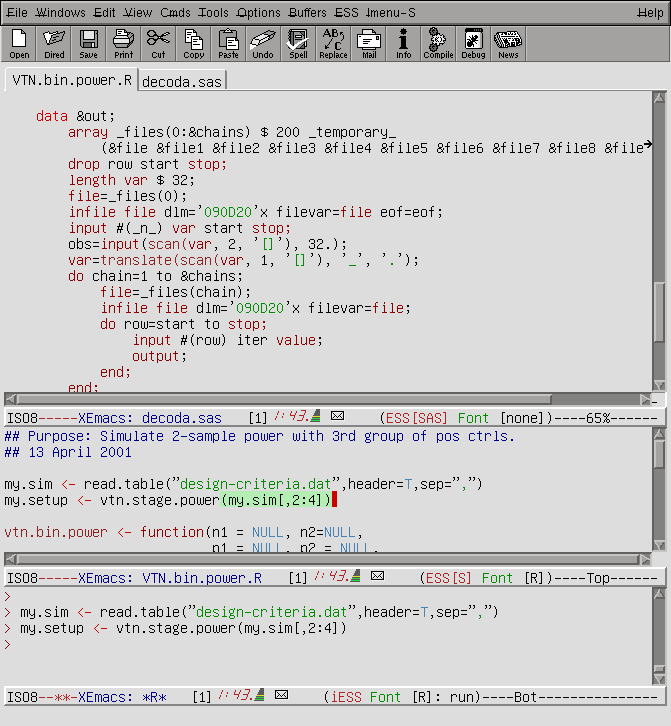
\includegraphics[height=7.0in,width=6.0in]{ess-xemacs-fig-1}
    \caption{XEmacs and ESS}%Editing SAS and R code and evaluation with R.}
    \label{fig:1}
  \end{center}
\end{figure}

\begin{figure}[htbp]
  \begin{center}
%    \includegraphics[height=7.0in,width=6.0in]{ess-xemacs-fig-2}
    \caption{XEmacs and ESS}%Editing and running \Splus\ and R.}
    \label{fig:2}
  \end{center}
\end{figure}


\end{document}

%%% Local Variables:
%%% mode: latex
%%% End:

